\documentclass[12pt]{article}
\usepackage[dvipsnames]{xcolor}
\usepackage{graphicx}
\usepackage{amsmath}
\usepackage{amssymb}
\usepackage[color,matrix,frame,arrow,curve]{xy}
\begin{document}


\begin{figure}[h!]\centering
\begin{minipage}{.5\linewidth}
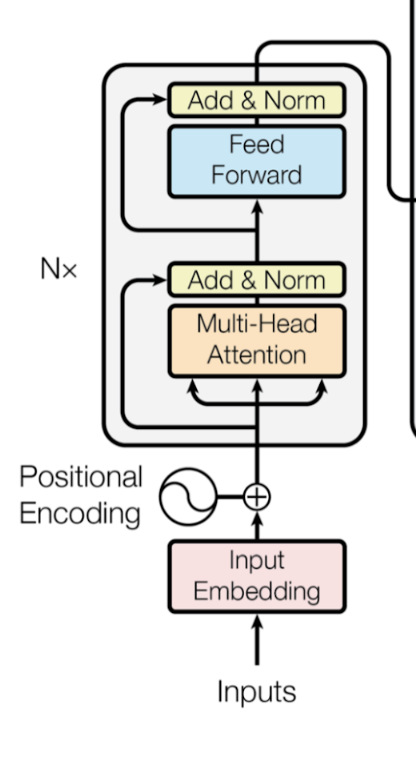
\includegraphics[width=2in]{encoder.jpg}
\end{minipage}%blank lines between minispaces breaks this
\begin{minipage}{.5\linewidth}
$$\xymatrix{
*+[F*:Dandelion]{\underline{q}^{3\times  4}}&*+[F*:Dandelion]{\underline{k}^{3\times  4}}&&
\\
*+[F*:yellow]{\underline{n}^{3\times  4}}\ar[u]\ar[ur]&&&
\\
&*+[F*:SkyBlue]{\underline{F}^{3\times  4}}\ar[ul]&&
\\
*+[F*:yellow]{\underline{N}^{3\times  4}}\ar[uu]\ar[ur]&&&
\\
&&*+[F*:Dandelion]{\underline{O}^{3\times  4}}\ar[ull]&
\\
&*+[F*:Dandelion]{\underline{Q}^{3\times  4}}\ar[ur]&*+[F*:Dandelion]{\underline{K}^{3\times  4}}\ar[u]&*+[F*:Dandelion]{\underline{V}^{3\times  4}}\ar[ul]
\\
*+[F*:gray]{\underline{p}^{3\times  4}}\ar[uuu]\ar[ur]\ar[urr]\ar[urrr]&&&
\\
*+[F*:Lavender]{\underline{R}^{3\times  4}}\ar[u]&&&
}$$
\end{minipage}
\caption{Encoder.}
\label{fig-texnn-for-encoder}
\end{figure}\begin{subequations}
\begin{equation}
q^{3\times  4} = n^{3\times  4})
\label{eq-q-fun-encoder}
\end{equation}

\begin{equation}
k^{3\times  4} = n^{3\times  4})
\label{eq-k-fun-encoder}
\end{equation}

\begin{equation}
n^{3\times  4} = N^{3\times  4},F^{3\times  4})
\label{eq-n-fun-encoder}
\end{equation}

\begin{equation}
F^{3\times  4} = N^{3\times  4})
\label{eq-F-fun-encoder}
\end{equation}

\begin{equation}
N^{3\times  4} = p^{3\times  4},O^{3\times  4})
\label{eq-N-fun-encoder}
\end{equation}

\begin{equation}
O^{3\times  4} = Q^{3\times  4},K^{3\times  4},V^{3\times  4})
\label{eq-O-fun-encoder}
\end{equation}

\begin{equation}
Q^{3\times  4} = p^{3\times  4})
\label{eq-Q-fun-encoder}
\end{equation}

\begin{equation}
K^{3\times  4} = p^{3\times  4})
\label{eq-K-fun-encoder}
\end{equation}

\begin{equation}
V^{3\times  4} = p^{3\times  4})
\label{eq-V-fun-encoder}
\end{equation}

\begin{equation}
p^{3\times  4} = R^{3\times  4})
\label{eq-p-fun-encoder}
\end{equation}

\begin{equation}
R^{3\times  4} =)
\label{eq-R-fun-encoder}
\end{equation}

\end{subequations}


\end{document}  
